% Slide graphics for the BTP progress deck: step-by-step derivation panels and
% diagrams, one per page.  Compile with pdflatex; report/render_slides.py turns
% each page into a transparent PNG for the Canva deck.
\documentclass[border=8pt,multi=page]{standalone}
\usepackage{lmodern}
\usepackage[T1]{fontenc}
\renewcommand{\familydefault}{\sfdefault}
\usepackage{amsmath,amssymb,bm}
\usepackage[dvipsnames]{xcolor}
\usepackage{tikz}
\usetikzlibrary{arrows.meta,patterns,calc,decorations.pathreplacing}
\usepackage[most]{tcolorbox}

\definecolor{navy}{HTML}{1F4E79}
\definecolor{ink}{HTML}{17324D}
\definecolor{corr}{HTML}{C0392B}
\definecolor{acc}{HTML}{E4572E}
\definecolor{soft}{HTML}{EAF1F8}
\newcommand{\rp}{r_p}
\newcommand{\Izz}{I_{zz}}
\newcommand{\tmin}{t_{\min}}
\newcommand{\tmax}{t_{\max}}
\newcommand{\fix}[1]{\textcolor{corr}{#1}}

% one derivation step: number, words, then the maths
\newcounter{stp}
\newcommand{\step}[2]{%
  \stepcounter{stp}%
  \par\noindent
  
\begin{tikzpicture}[baseline=(n.base)]
    \node(n)[circle,fill=navy,text=white,font=\bfseries\normalsize,inner sep=0pt,minimum size=1.5em]{\arabic{stp}};
  \end{tikzpicture}\hspace{0.6em}%
  \begin{minipage}[t]{0.93\linewidth}\leavevmode\color{ink}#1\end{minipage}\par
  \vspace{0.1em}{\color{ink}#2}\vspace{0.5em}}
\newtcbox{\result}{on line,colback=soft,colframe=navy,boxrule=0.8pt,arc=3pt,
  left=6pt,right=6pt,top=3pt,bottom=3pt}
\newcommand{\correction}[1]{\par\noindent\hspace*{2.1em}\begin{minipage}[t]{0.93\linewidth}\leavevmode\color{corr}\small\textbf{Correction to the notes:} #1\end{minipage}\par\vspace{0.5em}}
\newenvironment{panel}{\begin{page}\begin{minipage}{16.5cm}\setcounter{stp}{0}\large}{\end{minipage}\end{page}}

\begin{document}

% =====================================================================
% PANEL 1: area and neutral axis
\begin{panel}
\step{Treat the section as the outer disc minus the cavity disc.}
{\[A = \pi R^2 - \pi r^2 = \pi\,(R^2-r^2)\]}
\step{The centroid of a composite area is $\sum A_i y_i / \sum A_i$. The outer disc is centred at $y=0$;
the cavity is a \emph{negative} area centred at $y=\rp$.}
{\[\bar y = \frac{\pi R^2\cdot 0 \;-\; \pi r^2\cdot \rp}{\pi R^2-\pi r^2}\]}
\step{Cancel $\pi$. Material is missing on the $+y$ side, so the neutral axis moves toward the thick wall ($\bar y<0$).}
{\[\result{$\displaystyle \bar y = -\,\frac{r^2\,\rp}{\fix{R^2-r^2}}$}\]}
\correction{the notes have $R^2-r$ in the denominator; $r^2\rp/(R^2-r)$ is not even a length.}
\step{Placeholder design ($R=10$, $r=4$, $\rp=3$ mm):}
{\[A = 263.9\ \text{mm}^2,\qquad \bar y = -0.571\ \text{mm}\]}
\end{panel}

% =====================================================================
% PANEL 2: second moment of area
\begin{panel}
\step{Parallel-axis theorem, $I = I_c + A\,d^2$, for each disc about the neutral axis.
Distances: outer disc $d=|\bar y|$, cavity $d=\rp-\bar y$.}
{\[\Izz = \Big[\tfrac{\pi R^4}{4} + \pi R^2\,\bar y^{\,2}\Big] - \Big[\tfrac{\pi r^4}{4} + \pi r^2\,(\rp-\bar y)^2\Big]\]}
\step{A shortcut we use again later: the cavity distance simplifies to}
{\[\rp-\bar y = \rp + \frac{r^2\rp}{R^2-r^2} = \frac{R^2\,\rp}{R^2-r^2}\]}
\step{Substitute $\bar y$ and $\rp-\bar y$ into the two $A\,d^2$ terms and factor:}
{\[\pi R^2\bar y^{\,2}-\pi r^2(\rp-\bar y)^2=\frac{\pi\rp^2\,(R^2r^4-r^2R^4)}{(R^2-r^2)^2}=-\,\frac{\pi R^2 r^2 \rp^2}{R^2-r^2}\]}
\step{Result: concentric hollow tube, minus the stiffness lost by moving the hole off-centre.}
{\[\result{$\displaystyle \Izz = \frac{\pi\,(R^4-r^4)}{4} - \frac{\pi R^2 r^2 \rp^2}{R^2-r^2}$}
\qquad = 7652.9 - 538.6 = 7114\ \text{mm}^4\]}
\end{panel}

% =====================================================================
% PANEL 3: loading
\begin{panel}
\step{Pressure acts on the inside face of the sealed tip, whose area is the cavity area $A_c=\pi r^2$:}
{\[F = P\,\fix{A_c} = P\,\pi r^2\]}
\correction{the notes write $F=PA$, but $A$ already means the silicone area $\pi(R^2-r^2)$.}
\step{A uniform pressure on a circle has its resultant at the centre of the circle, $y=\rp$.
Its lever arm about the neutral axis (step 2 of the previous slide):}
{\[e = \rp-\bar y = \frac{R^2\,\rp}{R^2-r^2}\]}
\step{Moment = force $\times$ lever arm:}
{\[\result{$\displaystyle M = F\,e = \frac{\pi P R^2 r^2 \rp}{R^2-r^2}$}\]}
\step{Why $M$ is the same everywhere: cut at any $x$, keep the tip piece \emph{with its fluid}.
Only the cut carries load, so}
{\[\int_A \sigma_x\,dA = P\pi r^2,\qquad \int_A \sigma_x\,(y-\rp)\,dA = 0\]}
\step{Numbers: per kPa of pressure $F = 0.050$ N and $M = 0.180$ N\,mm.}{}
\end{panel}

% =====================================================================
% PANEL 4: beam response
\begin{panel}
\step{Euler--Bernoulli: plane sections stay plane and every fibre is in uniaxial stress,
$\sigma_x = E\,[\varepsilon_0+\kappa\,(y-\bar y)]$. Taking moments about the neutral axis gives}
{\[M = E\,\Izz\,\kappa \quad\Longrightarrow\quad \kappa = \frac{M}{E\,\Izz} = \frac{\pi P R^2 r^2 \rp}{E\,\Izz\,(R^2-r^2)}\]}
\step{$M$ is uniform, so $\kappa$ is uniform: the centreline is a circular arc of radius $\rho=1/\kappa$, and the tip turns by}
{\[\result{$\displaystyle \theta = \kappa\,l = \frac{\pi \fix{P} R^2 r^2 \rp\, l}{E\,\Izz\,(R^2-r^2)}$}\]}
\correction{the notes write $P^2$ here; $\theta=\kappa l$ is linear in $P$. Use the small-strain $E=3\mu$, not a secant modulus.}
\step{Arc geometry (figure): the tip moves sideways by}
{\[\delta = \rho\,(1-\cos\theta) = \frac{1-\cos\theta}{\kappa}\]}
\step{For small angles $1-\cos\theta\approx\theta^2/2$, which recovers the cantilever result:}
{\[\delta \approx \frac{\theta\,l}{2} = \frac{M\,l^2}{2E\Izz}\qquad(20\ \text{kPa: }\theta = 4.82^\circ,\ \delta = 4.20\ \text{mm})\]}
\end{panel}

% =====================================================================
% PANEL 5: (1 - 2 nu)
\begin{panel}
\step{The beam model ignores the wall stresses \emph{in the section plane} (radial $\sigma_r$, hoop $\sigma_\theta$).
Put them back with the full Hooke's law:}
{\[\varepsilon_x = \frac{\sigma_x-\nu(\sigma_y+\sigma_z)}{E}
\;\Longrightarrow\; \sigma_x = E\,[\varepsilon_0+\kappa(y-\bar y)] + \nu\,(\sigma_y+\sigma_z)\]}
\step{We never need the in-plane field itself. Equilibrium plus the divergence theorem gives its
total and where it acts: $2P\pi r^2$, through the cavity centre.}
{\[\int_A(\sigma_y+\sigma_z)\,dA = 2P\pi r^2,\qquad \int_A(\sigma_y+\sigma_z)(y-\bar y)\,dA = 2P\pi r^2\,e\]}
\step{Force balance on the cut (panel 3, step 4):}
{\[E A\,\varepsilon_0 + 2\nu P\pi r^2 = P\pi r^2 \;\Longrightarrow\; \varepsilon_0 = \fix{(1-2\nu)}\,\frac{P\pi r^2}{EA}\]}
\step{Moment balance on the cut:}
{\[E\Izz\,\kappa + 2\nu P\pi r^2 e = P\pi r^2 e \;\Longrightarrow\;
\result{$\displaystyle \kappa = \fix{(1-2\nu)}\,\frac{M}{E\,\Izz}$}\]}
\step{Silicone is incompressible, $\nu\to 0.5$: $\kappa\to 0$ and $\varepsilon_0\to 0$.
A bare actuator does \textbf{not} bend at first order. A hoop sleeve takes the hoop stress and restores $\kappa = M/(E\Izz)$.}{}
\end{panel}

% =====================================================================
% PANEL 6: wall thickness and the notes' linear wall-expansion term
\begin{panel}
\step{Draw a ray from the cavity centre $C$ at angle $\phi$ from $+y$. It leaves the outer circle at $Q$,
a distance $s=r+t$ from $C$. Law of cosines in triangle $OCQ$:}
{\[R^2 = \rp^2 + s^2 + 2\,\rp\, s\cos\phi\]}
\step{Solve the quadratic for $s$ (positive root) and subtract $r$:}
{\[\result{$\displaystyle t(\phi) = \sqrt{R^2-\rp^2\sin^2\fix{\phi}}\;-\;\rp\cos\phi\;-\;r$}
\qquad t(0)=\tmin=3,\ t(\pi)=\tmax=9\ \text{mm}\]}
\step{Thin-membrane hoop stress: the thin wall carries three times the hoop stress of the thick wall.}
{\[\sigma_\theta(\phi)\approx \frac{P\,r}{t(\phi)}\]}
\step{The notes assume a \emph{linear} axial strain $\varepsilon_x\propto Pr/(Et)$ and difference it across the section:}
{\[\kappa_{\exp}\approx\frac{\varepsilon_x(\text{thin})-\varepsilon_x(\text{thick})}{2R}=\frac{Pr}{2ER}\Big(\frac{1}{\tmin}\ \fix{-}\ \frac{1}{\tmax}\Big)\]}
\correction{the sign of the $1/\tmax$ term flips to $+$ when the notes substitute it into $\kappa_\text{total}$.}
\step{This cannot be added to $\kappa_\text{thrust}$: it uses the same linear Poisson coupling that, for $\nu=0.5$,
\emph{cancels} the thrust moment (previous slide). The real effect is second order (next slide).}{}
\end{panel}

% =====================================================================
% PANEL 7: second-order lengthening and the limit pressure
\begin{panel}
\step{Thin closed neo-Hookean tube. Hoop, axial and thickness stretches
$\lambda_1=1+a$, $\lambda_2=1+b$, $\lambda_3=1/(\lambda_1\lambda_2)$. Membrane stresses:}
{\[\sigma_\theta=\mu\,(\lambda_1^2-\lambda_3^2),\qquad \sigma_x=\mu\,(\lambda_2^2-\lambda_3^2)\]}
\step{A closed end carries half the hoop load axially, $\sigma_x=\sigma_\theta/2$:}
{\[2\lambda_2^2=\lambda_1^2+\lambda_3^2,\qquad \lambda_3^2\approx 1-2a-2b+3a^2+3b^2+4ab\]}
\step{First order in $a$: $4b=-2b$, so $b=0$. No linear lengthening, the same result as the $(1-2\nu)$ slide.}{}
\step{Second order, with $b=O(a^2)$: $6b=4a^2$, so}
{\[\result{$\displaystyle \varepsilon_\text{axial}\approx\tfrac{2}{3}\,\varepsilon_\text{hoop}^{\,2}$}\]}
\step{The thin wall has the larger hoop strain, so it lengthens more and the actuator curls toward the thick wall,
with $\kappa\propto P^2$ at low pressure (FE: slope 2). Past a limit the wall thins faster than its stress can rise:}
{\[P_\text{lim}=0.523\,\mu \qquad(104.7\ \text{kPa for } E=0.6\ \text{MPa})\]}
\end{panel}

% =====================================================================
% DIAGRAM A: actuator schematic (side view + section)
\begin{page}
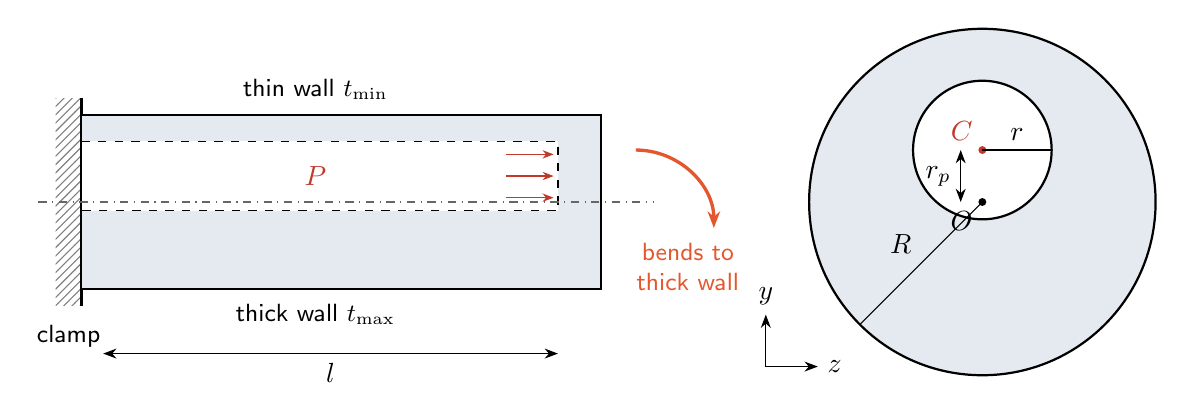
\begin{tikzpicture}[scale=1.1]
  \fill[pattern=north east lines,pattern color=black!50] (-0.3,-1.2) rectangle (0,1.2);
  \draw[thick] (0,-1.2) -- (0,1.2);
  \fill[navy!12] (0,-1) rectangle (6,1);
  \draw[thick] (0,1) -- (6,1) -- (6,-1) -- (0,-1);
  \fill[white] (0,-0.1) rectangle (5.5,0.7);
  \draw[dashed] (0,0.7) -- (5.5,0.7) -- (5.5,-0.1) -- (0,-0.1);
  \draw[dash dot,black!60] (-0.5,0) -- (6.6,0);
  \foreach \y in {0.05,0.3,0.55} \draw[-{Stealth[length=4pt]},corr] (4.9,\y) -- (5.45,\y);
  \node[corr] at (2.7,0.3) {$P$};
  \node[font=\small] at (2.7,1.3) {thin wall $\tmin$};
  \node[font=\small] at (2.7,-1.3) {thick wall $\tmax$};
  \draw[{Stealth}-{Stealth}] (0.25,-1.75) -- (5.5,-1.75) node[midway,below] {$l$};
  \node[font=\small] at (-0.15,-1.55) {clamp};
  \draw[-{Stealth[length=6pt]},very thick,acc] (6.4,0.6) arc[start angle=90,end angle=0,radius=0.9];
  \node[acc,font=\small,align=center] at (7.0,-0.75) {bends to\\thick wall};
  \begin{scope}[shift={(10.4,0)}]
  \fill[navy!12] (0,0) circle (2);
  \draw[thick] (0,0) circle (2);
  \fill[white] (0,0.6) circle (0.8);
  \draw[thick] (0,0.6) circle (0.8);
  \fill (0,0) circle (1.3pt) node[below left] {$O$};
  \fill[corr] (0,0.6) circle (1.3pt) node[above left,corr] {$C$};
  \draw (0,0.6) -- (0.8,0.6) node[midway,above] {$r$};
  \draw (0,0) -- (-1.414,-1.414) node[midway,above left] {$R$};
  \draw[{Stealth}-{Stealth}] (-0.25,0) -- (-0.25,0.6) node[midway,left] {$\rp$};
  \draw[-{Stealth}] (-2.5,-1.9) -- (-1.9,-1.9) node[right] {$z$};
  \draw[-{Stealth}] (-2.5,-1.9) -- (-2.5,-1.3) node[above] {$y$};
  \end{scope}
\end{tikzpicture}
\end{page}

% =====================================================================
% DIAGRAM B: section with neutral axis, ybar, e and parallel-axis distances
\begin{page}
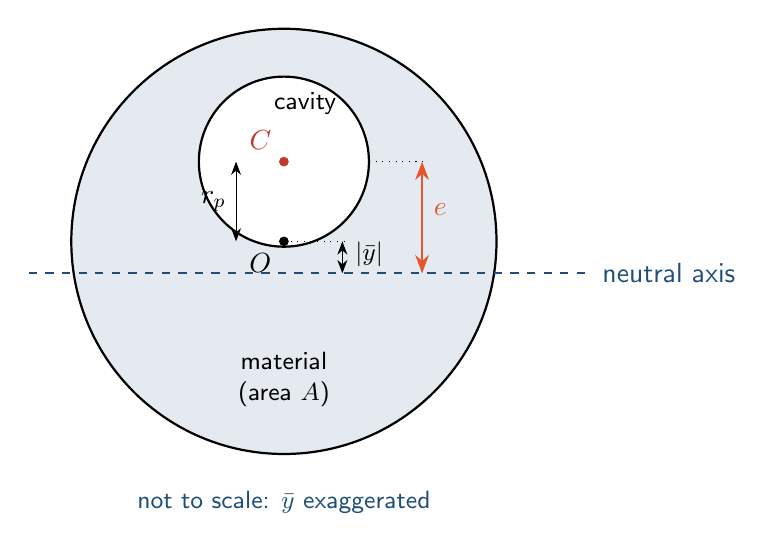
\begin{tikzpicture}[scale=1.35]
  \fill[navy!12] (0,0) circle (2);
  \draw[thick] (0,0) circle (2);
  \fill[white] (0,0.75) circle (0.8);
  \draw[thick] (0,0.75) circle (0.8);
  \fill (0,0) circle (1.3pt) node[below left=1pt] {$O$};
  \fill[corr] (0,0.75) circle (1.3pt) node[above left=1pt,corr] {$C$};
  \draw[dashed,navy,thick] (-2.4,-0.3) -- (2.9,-0.3) node[right] {neutral axis};
  \draw[{Stealth}-{Stealth}] (0.55,0) -- (0.55,-0.3);
  \node[right,font=\small] at (0.58,-0.12) {$|\bar y|$};
  \draw[{Stealth}-{Stealth},acc,thick] (1.3,-0.3) -- (1.3,0.75);
  \node[acc,right] at (1.32,0.3) {$e$};
  \draw[dotted] (0.8,0.75) -- (1.35,0.75);
  \draw[dotted] (0,0) -- (0.6,0);
  \draw[{Stealth}-{Stealth}] (-0.45,0) -- (-0.45,0.75) node[midway,left] {$\rp$};
  \node[font=\small,align=center] at (0,-1.3) {material\\(area $A$)};
  \node[font=\small,align=center] at (0.2,1.3) {cavity};
  \node[font=\small,align=center,navy] at (0,-2.45) {not to scale: $\bar y$ exaggerated};
\end{tikzpicture}
\end{page}

% =====================================================================
% DIAGRAM C: free body
\begin{page}
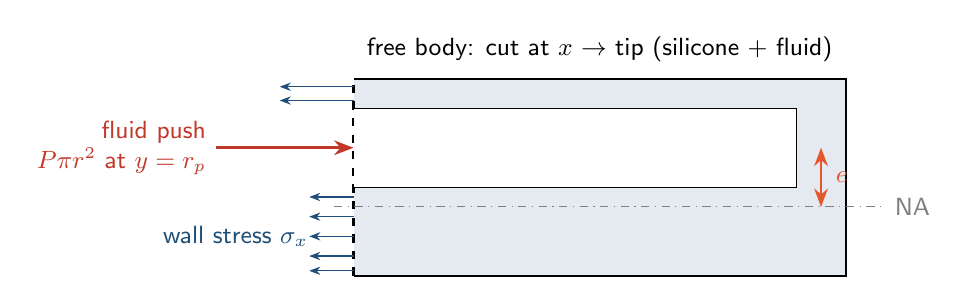
\begin{tikzpicture}[scale=1.25]
  \fill[navy!12] (0,-1) rectangle (5,1);
  \draw[thick] (0,1) -- (5,1) -- (5,-1) -- (0,-1);
  \draw[thick,dashed] (0,-1) -- (0,1);
  \fill[white] (0,-0.1) rectangle (4.5,0.7);
  \draw (0,0.7) -- (4.5,0.7) -- (4.5,-0.1) -- (0,-0.1);
  \node[font=\small] at (2.5,1.3) {free body: cut at $x$ $\to$ tip (silicone + fluid)};
  \draw[-{Stealth[length=7pt]},very thick,corr] (-1.4,0.3) -- (0,0.3);
  \node[corr,left,font=\small,align=right] at (-1.4,0.3) {fluid push\\$P\pi r^2$ at $y=\rp$};
  \foreach \y in {0.78,0.92} \draw[-{Stealth[length=4pt]},navy] (0,\y) -- (-0.75,\y);
  \foreach \y in {-0.2,-0.4,-0.6,-0.8,-0.95} \draw[-{Stealth[length=4pt]},navy] (0,\y) -- (-0.45,\y);
  \node[navy,font=\small] at (-1.2,-0.6) {wall stress $\sigma_x$};
  \draw[dash dot,black!50] (-0.2,-0.3) -- (5.4,-0.3) node[right,font=\small] {NA};
  \draw[{Stealth}-{Stealth},acc,thick] (4.75,-0.3) -- (4.75,0.3);
  \node[acc,right,font=\small] at (4.8,0.0) {$e$};
\end{tikzpicture}
\end{page}

% =====================================================================
% DIAGRAM D: arc geometry
\begin{page}
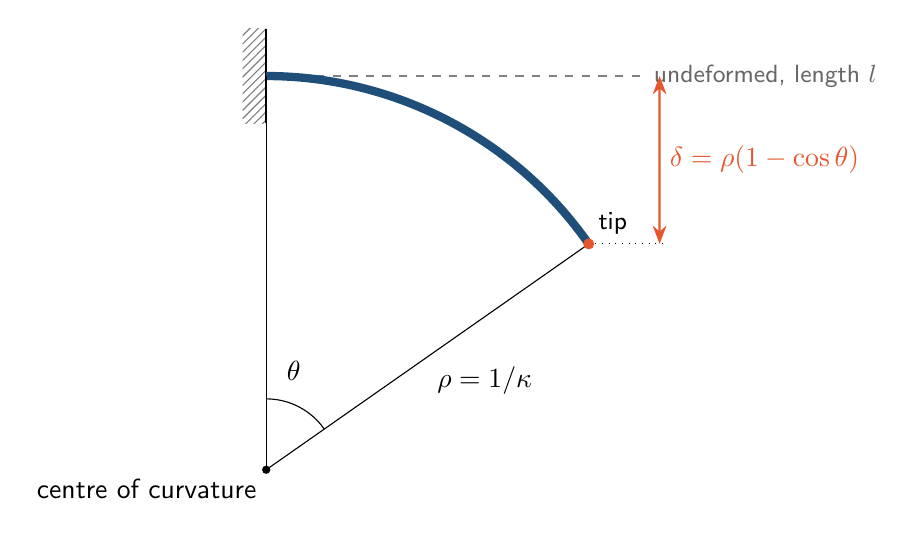
\begin{tikzpicture}[scale=1.0]
  \def\rr{5}\def\th{55}
  \fill[pattern=north east lines,pattern color=black!50] (-0.3,-0.6) rectangle (0,0.6);
  \draw[thick] (0,-0.6) -- (0,0.6);
  \draw[dashed,black!50] (0,0) -- ({\rr*rad(\th)},0) node[right,black!60,font=\small] {undeformed, length $l$};
  \draw[line width=3pt,navy] (0,0) arc[start angle=90,end angle={90-\th},radius=\rr];
  \coordinate (T) at ({\rr*sin(\th)},{-\rr*(1-cos(\th))});
  \coordinate (Cc) at (0,-\rr);
  \fill (Cc) circle (1.5pt) node[below left] {centre of curvature};
  \draw[thin] (Cc) -- (0,0);
  \draw[thin] (Cc) -- (T) node[midway,below right] {$\rho=1/\kappa$};
  \draw (0,-\rr+0.9) arc[start angle=90,end angle={90-\th},radius=0.9];
  \node at ({0.35},{-\rr+1.25}) {$\theta$};
  \draw[{Stealth}-{Stealth},acc,thick] ($(T)+(0.9,0)$) -- ({\rr*sin(\th)+0.9},0) node[midway,right] {$\delta=\rho(1-\cos\theta)$};
  \draw[dotted] (T) -- ($(T)+(1.0,0)$);
  \fill[acc] (T) circle (2pt);
  \node[above right,font=\small] at (T) {tip};
\end{tikzpicture}
\end{page}

% =====================================================================
% DIAGRAM E: in-plane stresses in the wall
\begin{page}
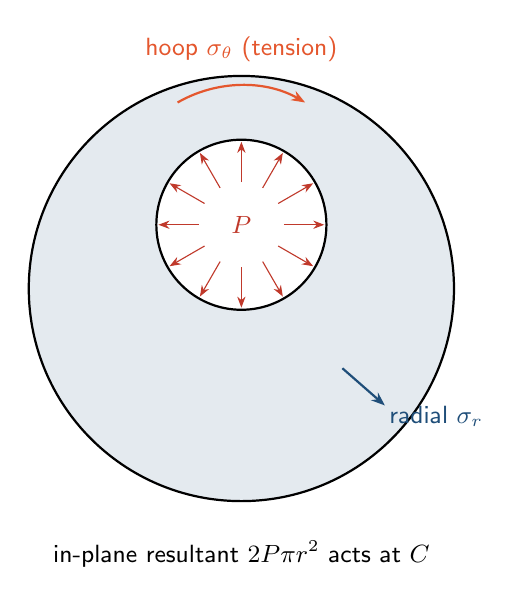
\begin{tikzpicture}[scale=1.35]
  \fill[navy!12] (0,0) circle (2);
  \draw[thick] (0,0) circle (2);
  \fill[white] (0,0.6) circle (0.8);
  \draw[thick] (0,0.6) circle (0.8);
  \foreach \a in {0,30,...,330} \draw[-{Stealth[length=4pt]},corr] ($(0,0.6)+(\a:0.4)$) -- ($(0,0.6)+(\a:0.78)$);
  \node[corr,font=\small] at (0,0.6) {$P$};
  \draw[-{Stealth[length=5pt]},acc,thick] (-0.6,1.75) arc[start angle=120,end angle=60,radius=1.2];
  \node[acc,font=\small] at (0,2.25) {hoop $\sigma_\theta$ (tension)};
  \draw[-{Stealth[length=5pt]},navy,thick] (0.95,-0.75) -- (1.35,-1.1);
  \node[navy,font=\small,right] at (1.3,-1.2) {radial $\sigma_r$};
  \node[font=\small,align=center] at (0,-2.5) {in-plane resultant $2P\pi r^2$ acts at $C$};
\end{tikzpicture}
\end{page}

% =====================================================================
% DIAGRAM F: wall thickness along a ray
\begin{page}
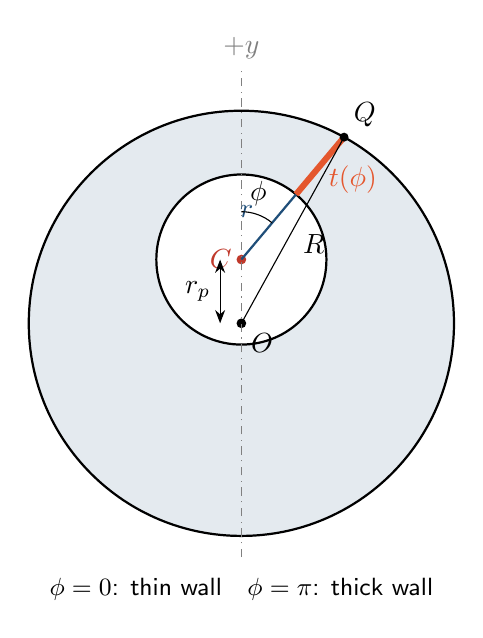
\begin{tikzpicture}[scale=1.35]
  \fill[navy!12] (0,0) circle (2);
  \draw[thick] (0,0) circle (2);
  \fill[white] (0,0.6) circle (0.8);
  \draw[thick] (0,0.6) circle (0.8);
  \fill (0,0) circle (1.3pt) node[below right] {$O$};
  \fill[corr] (0,0.6) circle (1.3pt) node[left,corr] {$C$};
  \draw[dash dot,black!50] (0,-2.2) -- (0,2.4) node[above] {$+y$};
  \draw[thick,navy] (0,0.6) -- (0.5142,1.2128);
  \draw[line width=2.2pt,acc] (0.5142,1.2128) -- (0.9661,1.7513);
  \draw (0,0) -- (0.9661,1.7513);
  \node[navy] at (0.05,1.05) {$r$};
  \node[acc] at (1.05,1.35) {$t(\phi)$};
  \node at (0.68,0.75) {$R$};
  \draw (0,1.05) arc[start angle=90,end angle=50,radius=0.45];
  \node at (0.16,1.22) {$\phi$};
  \fill (0.9661,1.7513) circle (1.2pt) node[above right] {$Q$};
  \draw[{Stealth}-{Stealth}] (-0.2,0) -- (-0.2,0.6) node[midway,left] {$\rp$};
  \node[font=\small] at (0,-2.5) {$\phi=0$: thin wall\quad $\phi=\pi$: thick wall};
\end{tikzpicture}
\end{page}

% =====================================================================
% TABLE: the twelve corrections
\begin{page}
\begin{minipage}{24cm}\large\color{ink}
\renewcommand{\arraystretch}{1.55}
\begin{tabular}{@{}r l l l l@{}}
\color{navy}\bfseries \# & \color{navy}\bfseries Where & \color{navy}\bfseries In the notes & \color{navy}\bfseries Corrected & \color{navy}\bfseries Why\\\hline
1 & p.\,1, eq.\,2 & $\bar y=-r^2\rp/(R^2-r)$ & $\bar y=-r^2\rp/(\fix{R^2-r^2})$ & typo; not a length\\
2 & p.\,2, eq.\,4 & $F=PA$ & $F=P\,\fix{A_c}=P\pi r^2$ & $A$ is the silicone area\\
3 & p.\,3, $\theta$ & $\theta\propto P^2$ & $\theta\propto \fix{P}$ & $\theta=\kappa l$; units\\
4 & p.\,3, eq.\,7 & $E$ = Young's or secant & small-strain $E=3\mu=6C_{10}$ & nonlinearity is ballooning\\
5 & pp.\,2--4 & beam formula, any actuator & only with \fix{hoop reinforcement} & in-plane stresses ignored\\
6 & bare actuator & $\kappa = M/(E\Izz)$ & $\kappa=\fix{(1-2\nu)}\,M/(E\Izz)\approx 0$ & incompressible silicone\\
7 & p.\,4, note (b) & $\Delta l=Fl/(EA)$, NA shifts & bare: $\Delta l\approx 0$; \fix{no NA shift} & uniform strain\\
8 & p.\,4, note (a) & strain-dependent $E$ in beam & hyperelastic law in FE / Tier 3 & different mechanism\\
9 & p.\,5, $t(\phi)$ & $\sin^2\theta$, mixed angles & $\sin^2\fix{\phi}$, $\phi$ from $+y$, exact & one angle\\
10 & pp.\,5--6 & $\varepsilon_{zz}$, $\sigma_z$ axial & $\fix{\varepsilon_x}$, $\fix{\sigma_x}$ & axis is $x$\\
11 & p.\,6, $\kappa_\text{total}$ & $+\,1/\tmax$ & $\fix{-}\,1/\tmax$ & sign of the definition\\
12 & pp.\,6--7 & $\kappa_{\exp}$ linear in $P$, added & $\varepsilon_\text{ax}\approx\tfrac23\varepsilon_\text{hoop}^2$; ends in a limit & second-order effect\\\hline
\end{tabular}
\end{minipage}
\end{page}

\end{document}
